%-------------------------
% Usage Examples: Industry
%-------------------------

  \subsection*{Industry}
    \label{industry}

    Due to the breadth and maturity of its code base, as well as the its commercial-friendly license, scikit-image is well suited for industrial applications.

    BT Imaging \citep{BTImaging} designs and builds tools that use photoluminescence (PL) imaging for photovoltaic applications. PL imaging can characterize the quality of multicrystalline silicon wafers by illuminating defects that are not visible under standard viewing conditions. The left panel of Figure \ref{fig:PL} shows an optical image of a silicon wafer, and the center panel shows the same wafer using PL imaging. In the right panel, the wafer defects and impurities have been detected through automated image analysis. scikit-image plays a key role in the image processing pipeline. For example, a Hough transform (\texttt{transform.hough\_line}) finds the wafer edges in order to segment the wafer from the background. scikit-image is also used for feature extraction. Crystal defects (dislocations) are detected using a band-pass filter, which is implemented as a Difference of Gaussians (\texttt{filter.gaussian\_filter}).

    The image processing results are input to machine learning algorithms, which assess intrinsic wafer quality. Solar cell manufacturers can use this information to reject poor quality wafers and charge more for cells that are expected to have high efficiency.

    \begin{figure*}[bht]

      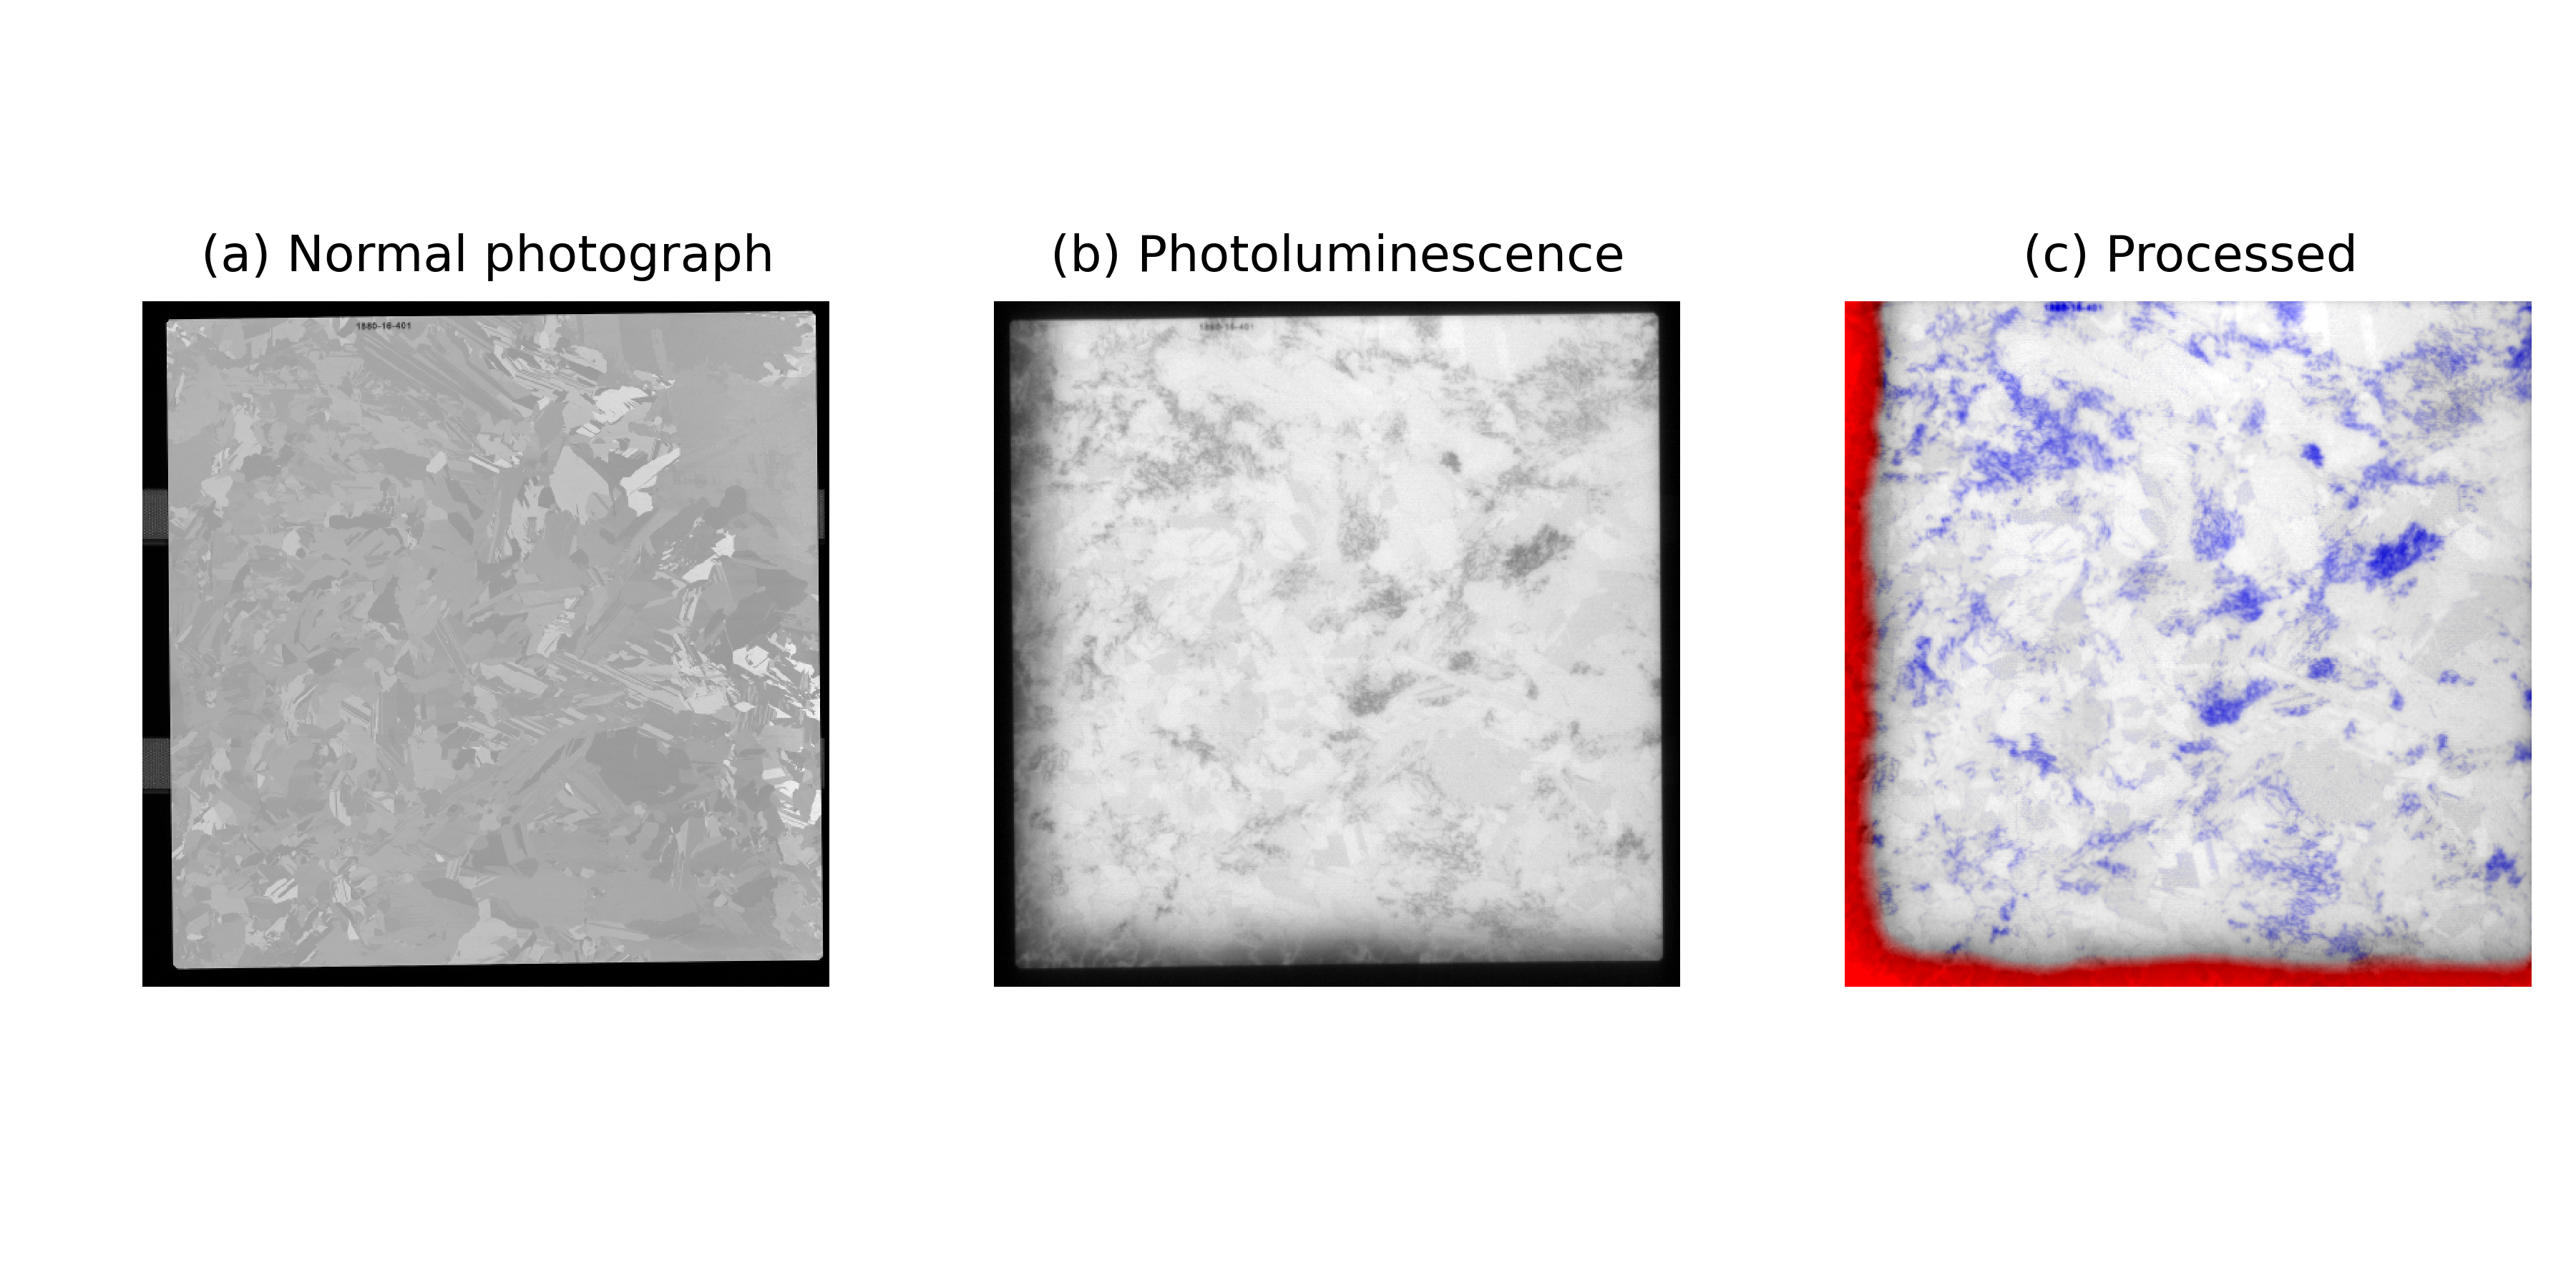
\includegraphics[width=\columnwidth]{fig_pl.png}

      \caption{\textit{Left}: An image of an as-cut silicon wafer before it has been processed into a solar cell. \textit{Center}: A PL image of the same wafer. Wafer defects, which have a negative impact solar cell efficiency, are visible as dark regions. \textit{Right}: Image processing results. Defects in the crystal growth (dislocations) are colored blue, while red indicates the presence of impurities. \label{fig:PL}}
    \end{figure*}

    scikit-image is also applied in a commercial setting for biometric security applications. AICBT Ltd uses multispectral imaging to detect when a person attempts to conceal their identity using a facial mask \citep{AICBT}. scikit-image performs file I/O (\texttt{io.imread}), histogram equalization (\texttt{exposure.equalize\_hist}), and aligns a visible wavelength image with a thermal image (\texttt{transform.AffineTransform}). The system determines the surface temperature of a subject's skin and detects situations where the face is being obscured.
